\documentclass{article}
\usepackage{epsfig}
\usepackage{graphicx}
%\usepackage[a4paper, total={6in, 10in}]{geometry}
\usepackage[table]{xcolor}
\usepackage{tikz}
\title{CS345 Theoretical Assignment 1 \\ }
\author{\vspace{2mm} \large Ayush Agarwal, 13180 \\ M.Arunothia, 13378}
\date{}
\begin{document}
\maketitle
\tableofcontents
\newpage
\section{Non-Dominated Points}
\subsection{Overview}
Given a set of coordinates P, we create list of each layer in the following manner.\\
First sort the coordinates based on Y-coordinate in descending order. Then maintain an array A of size $n$. Start with the first coordinate from 
the sorted array P(of all coordinates). This point will be a non-dominated point and will be a part of layer 1. Update the first index of A with the x-coordinate
of this point. Now take the second point from P. If its x coordinate is greater than the x-coordinate of earlier point, it means that it will be part of layer
1. If so then add it to layer 1 and update the layer 1's index in A. Otherwise it will be in second layer, so add it in layer 2 and update the layer 2's index 
in A with it's x coordinate. Repeat the above procedure for all points.

\subsection{Pseudo-Code}
Non-Dominated-points(P)	\\*
\{			\\*
    \hspace*{1cm}$ P  \longrightarrow  reverse\_sort(P)$ //sort in descending order of Y  \\*
    \hspace*{1cm} $ Layer[n]; A[n] $\\*
    \hspace*{1cm} $ A[0]=P[0].x $\\*
    \hspace*{1cm} $Layer[1].push(P[0])$ \\*
	\hspace*{1cm} $i=1; right=1 $\\*
    \hspace*{1cm} $while(i < P.length())$\\*
    \hspace*{2cm} $point = P[i]$\\*
    \hspace*{2cm} $index = binary\_search\_predecessor(A, 0, right, point.x)$ \\*
    \hspace*{4cm}                // returns the predecessor's index \\*
    \hspace*{2cm} $Layer[index].push(point)$\\*
    \hspace*{2cm} $A[index] = point.x$\\*
    \hspace*{2cm} $If (index > right ) right++ $\\*
	\hspace*{1cm} $return  Layer $\\*
	\\*
\} \\
\\
binary\_search\_predecessor(A, left, right, x)
\{ \\*
\hspace*{1cm} If no entry in A is less than x, return $right+1$ \\*
			 else return the index of maximum x coordinate less than x. \\*
\} \\*

\subsection{Time Complexity}
  Sorting step takes $O(nlogn)$ time, followed by binary\_search for each point which takes maximum $ logn $ time per point.
  $while$ iterates for all the points and in each iteration binary\_search is invoked, thus the loop takes $ n*logn $ time.
  Overall algorithm takes time \\
             $O(nlogn) + O(nlogn) = O(nlogn) $
\subsection{Proof of Correctness}
\subsubsection{What is to be proved?}
As we go along the iterations, say we have covered k points then, we have partially constructed layers. If the new $k+1$th point lies between the $i$th and $i+1$th (that is the $x$ predecessor of $k+1$ is the last point encountered in layer $i$) of these layers then it has to belong to layer $i$.
\subsubsection{Reasoning by Contradiction}
\begin{itemize}
\item It cannot belong to any layer $>i$ as the layers are increasingly drawn in x.
\item It cannot belong to any layer $<i$ as this point is clearly not dominated by the points in layer $i$ that is seen so far.
\item Hence, The point should belong to layer $i$.
\end{itemize}

\newpage
\section{ Open Rectangle Query }
\subsection{Data Structure Design : } 
Given an array 'a' of 'n' coordinate points, we construct a Binary Search Tree (BST) call it 'data' in the following manner.\\*
\begin{itemize}
\item Sort the array 'a' w.r.t the x-coordinates of the points. Call this sorted array 'b'.
\item Divide 'b' into $ \frac{n}{Log[n]} $ parts, starting from the beginning. Index each of the part incrementally from 1 to $ \frac{n}{Log[n]} $. 
\item Construct BST 'data' with $ \frac{n}{Log[n]} = N $ nodes from 'b' using the above indexing for the comparisons.
\item Now, we have a BST 'data' with 'N' nodes augmented with an array of $Log[n]$ size at every node and, also
    x\_min and x\_max of its $logn$ chunk. Sort this array at every node on basis of y-coordinates of the points.
\item Every node is augmented with another inversely sorted array of y\_max(maximum y coordinate of each logn size array)
    of each of the nodes belonging to the subtree, accompanied by a pointer to that node. 
    In short a node at level i from the bottom will be augmented with two arrays, one of size $logn$ say short\_array
    which contains the sorted array of according to y, other will be an array of size $2^i$ say long\_array.
\item This completes the description of augmented BST 'data'.
\end{itemize}

\subsection{Preprocessing : }
\begin{itemize}
\item[\bf STEP 1 : ]
Start
\item[\bf STEP 2 : ]
Make a bst as specified above with each node having $logn$ size sorted array of its chunk. For the other array
start traversing from the leaf node. 
The leaf node will have will have only one entry in its long\_array, i.e, the maximum y coordinate in its logn chunk,
and the pointer to itself. 
\item[\bf STEP 3 : ]
Now consider the parent node of this leaf node. It will have 3 entries in its long\_array in the sorted order, 
two from its children and the third from itself(which has a pointer to itself). 
\item[\bf STEP 4 : ]
    At any non-leaf node, merge the long\_array of its two children and its y\_max (as in merge sort).

\end{itemize}
\subsection{Pseudo Code : }

{\bf subtree\_points(node n, x1, x2, y\_bottom, flag)}\\
\{\\
    \hspace*{1cm}for i in n.long\_array:\\
    \hspace*{2cm}       if $i.y < y\_bottom$ :\\
    \hspace*{3cm}                        print\_points($*$ i.pointer, x1, x2, y\_bottom)\\            
\}\\
\\
{\bf print\_points(node n, x1, x2, y\_bottom, flag)}\\
\{\\
    \hspace*{1cm}  if $flag==1$:             //intermediate node \\
    \hspace*{1.5cm}for i in n.short\_array :\\
    \hspace*{2cm}    if(i $<$ y\_bottom) return;\\
    \hspace*{2cm}    else print i\\
    \hspace*{1cm}  else     //boundary node of the required range\\
    \hspace*{1.5cm}    for i in nth chunk in original array :\\
    \hspace*{2cm} if(x1 $<=$ i.x $<=$ x2 \&\& i.y $>=$ y\_bottom) print i \\*
\}\\

\emph{root} is the head of preprocessed binary tree \\
{\bf query($x1, x2$ , y\_bottom, root)}\\
\hspace*{1cm}if x2 $<$ root.x\_min\\
\hspace*{2cm}    query($x1, x2$ , y\_bottom, root.left)\\
\hspace*{1cm}else if x1 $>$ root.x\_max \\
\hspace*{2cm}    query($x1, x2$ , y\_bottom, root.right)\\
\hspace*{1cm}else if (x1, x2 belongs root) \\* 
\hspace*{2cm} print\_points(root, x1, x2, y\_bottom, 0) \\*  
\hspace*{1cm}else if (x1 belongs root) \\*
\hspace*{1.5cm} print\_points(root, x1, x2, y\_bottom, 1) \\*
\hspace*{1.5cm} binary\_search(x2, right, y\_bottom, root.right) \\*
\hspace*{1cm}else if (x2 belongs root) \\*
\hspace*{1.5cm} print\_points(root, x1, x2, y\_bottom, 1) \\*
\hspace*{1.5cm} binary\_search(x1, left, y\_bottom, root.left) \\*
\hspace*{1cm}else  \\*
\hspace*{2cm}binary\_search(x1,left, y\_bottom, root.left) \\*
\hspace*{2cm}binary\_search(x2,right, y\_bottom, root.right) \\*

\newpage
{\bf binary\_search ($x$, type, y\_bottom, root)}\\*
\hspace*{1cm} if(type $==$ "left") \\*
\hspace*{2cm}    if(x1 $<$ root.x\_min) \\*
\hspace*{3cm}    subtree\_points(root.right, x1, infinite, y\_bottom, 0) \\*
\hspace*{3cm}    binary($x$, left, y\_bottom, root.left) \\*
\hspace*{2cm}    else if (x1 belongs root) \\*
\hspace*{3cm}      print\_points(root, x1, infinite, y\_bottom, 0) \\*
\hspace*{2cm}    else binary\_search ($x$, right, y\_bottom, root.right)\\*
\hspace*{1cm}else \\*
\hspace*{2cm} repeat similarly for $type=="right"$

\subsection{Space Complexity : }
The data structure we invented, is a BST of size $N*(augmentation\_size)$.\\*
Therefore, space used is - (Refer Sub section Data Structure Design)
\begin{itemize}
\item Due to $x_{min}$,$x_{max}$ and flag augmentation - $N * O(1)$ \\*
\item Due to short\_array augmentation - $N * Log(n)$ \\*
\item Due to long\_array augmentation - at every level in the tree this augmentation takes $N$ space, implying a total of - $N * Log(n)$ \\*  
\item Thus, overall space complexity is = \\*
$O(N*Log(n)) = O(n)$ as $N = n/log(n)$.
\end{itemize}
\subsection{Time Complexity : }
\subsubsection{Query Time : }
\begin{itemize}
\item Locating the $x_1$ and $x_2$ in our BST takes O(Log(n)) time each.
\item As we have $long\_{array}$ to skip all those nodes which don't have any point in range, we precisely traverse only to those nodes which can yield us atleast one point that is to be reported. Moreover, in each such node, we traverse the $short\_array$ from max to till $>=y_{bottom}$ is satisfied and this keeps our search within the bounds of O(k).
\item Hence, overall time for a query is O(k+Log(n)). 
\end{itemize}
\subsubsection{Pre-processing Time : }
\begin{itemize}
\item The first sort based on x coordinates requires O(n*Log(n)).
\item The construction of BST with all its augmentation requires - \\*
$T(n) = 2*T(n/2) + an$ // O(n) to take care of the merging of the augmentations as described above \\*
= O(n*Log(n))
\item Hence, overall pre-processing requires O(n*log(n)).  

\end{itemize}
\subsection{Proof of Correctness}
\subsubsection{What is to be proved?}
\begin{itemize}
\item Every point in the given range of $(x_1,y_1)$ and $(x_2,y_2)$ is getting reported.
\item Every reported point is in the given range.
\end{itemize}
\subsubsection{Explanation}
\begin{itemize}
\item The array is getting sorted initially on the basis of x-coordinates and the chunks of $log(n)$ size are formed from this sorted array. The BST is constructed on these chunks based on their increasing x-range and hence, from the correctness of BST functioning, we are assured to get the correct x range when we traverse the BST on its basis.
\item From the augmentation of the BST, we see that every $short\_array$ is sorted within on the basis of y-coordinates. Hence, on traversing it from max to min order till $y>=y_{bottom}$ ensures that we report points only within range.
\item No point in the given range will get missed out as we do a search on the BST for x range (similar to one discussed in class) and as we traverse a sorted $short\_array$ till we satisfy $y>=y_{bottom}$. 
\item Hence, this proves the correctness of the algorithm. 
\end{itemize}
\newpage
\section{A real life application of Directed Acyclic Graphs}
\subsection{Overview}
This problem is approached by exploiting the topological ordering of DAGs. By the definition of root and exit, they will appear on the leftmost and rightmost ends of the ordering.
\subsection{Algorithm}
\begin{itemize}
\item Start.
\item Sort the vertices to get their topological ordering. Let $path$ be an array, defined as - $path[i]$ stores the number of distinct paths from root to the $i^{th}$ node in the topological ordering. Initialize all entries of this array with $0$.
\item Let $i = 1$, the first vertex after root in order. Run the following step till $i <> n-1$
\item For all incoming vertices to this $i^{th}$ node : edge ($node_j, node_i$) exists
\begin{itemize}
\item assign edge weight as $path[i]$
\item $path[i] += path[j]$
\end{itemize} 
\item Stop.
\end{itemize}
\subsection{Pseudo Code}
Assign\_edge\_weight(V,E)	\\*
\{			\\*
	\hspace*{1cm}node[ ] = topological\_sort(V,E) \\*
	\hspace*{1cm}path[ ] = $0$ \\*
	\hspace*{1cm} $i = node[1]$ // $node[0$] will be $root$\\*
	\hspace*{1cm} while$(i <> n-1)$  \\*
	\hspace*{2cm} For all $(node[j], node[i]) \in E$ \\*
	\hspace*{3cm} $w(node[j], node[i]) = path[i]$ \\*
	\hspace*{3cm} $path[i] += path[j]$ \\*
	\hspace*{1cm}return \\*
\}
\subsection{Time Complexity}
\begin{itemize}
\item Topological sorting - single DFS (using Finish Time) $= O(m+n)$
\item O(while\_loop) = O(sum of in degrees in the graph) $= O(m+n)$
\item Hence, overall time for a query is $O(m+n)$. 
\end{itemize}
\subsection{Proof of Correctness}
\subsubsection{What is to be proved? or Claim}
That given any square of side length 'n' (a power of 2)  and Prime Minister's office P we can exhaust the rest of the square with non overlapping pieces of L-shaped tiles ( L-shape containes 3 unit sqaures that can be guarded by a commando and hence is equivalent to the given problem).  \\*
\subsubsection{Proof by Induction}
Induction is carried out on the length of the square. \\*
\subsubsection{Base Cases}
\begin{itemize}
\item $(n<2)$ - No commandos needed. \\*
\item $(n==2)$ - Only one commando needed and he should be placed so as to cover 'L' shape that leaves out Prime Minister's cabin. \\*
\end{itemize}
\subsubsection{Hypothesis}
Let $ n = 2^{k} $. \\*
Let us assume that the Claim is true for all $i<=k$ where $k>1$ and both are integers. \\*
\subsubsection{Inductive Step}
Let us prove that claim for $ k+1 $ is true. \\*
The square of size $2^{k+1}$ can be broken into four squares of size $2^{k}$. As the claim holds for sizes $<=k$, these 4 squares can be exhausted in the required way, (i.e) PM cabin anywhere we chose it to be and the rest exhausted with non overlapping 'L' shapes. \\*
\begin{center}
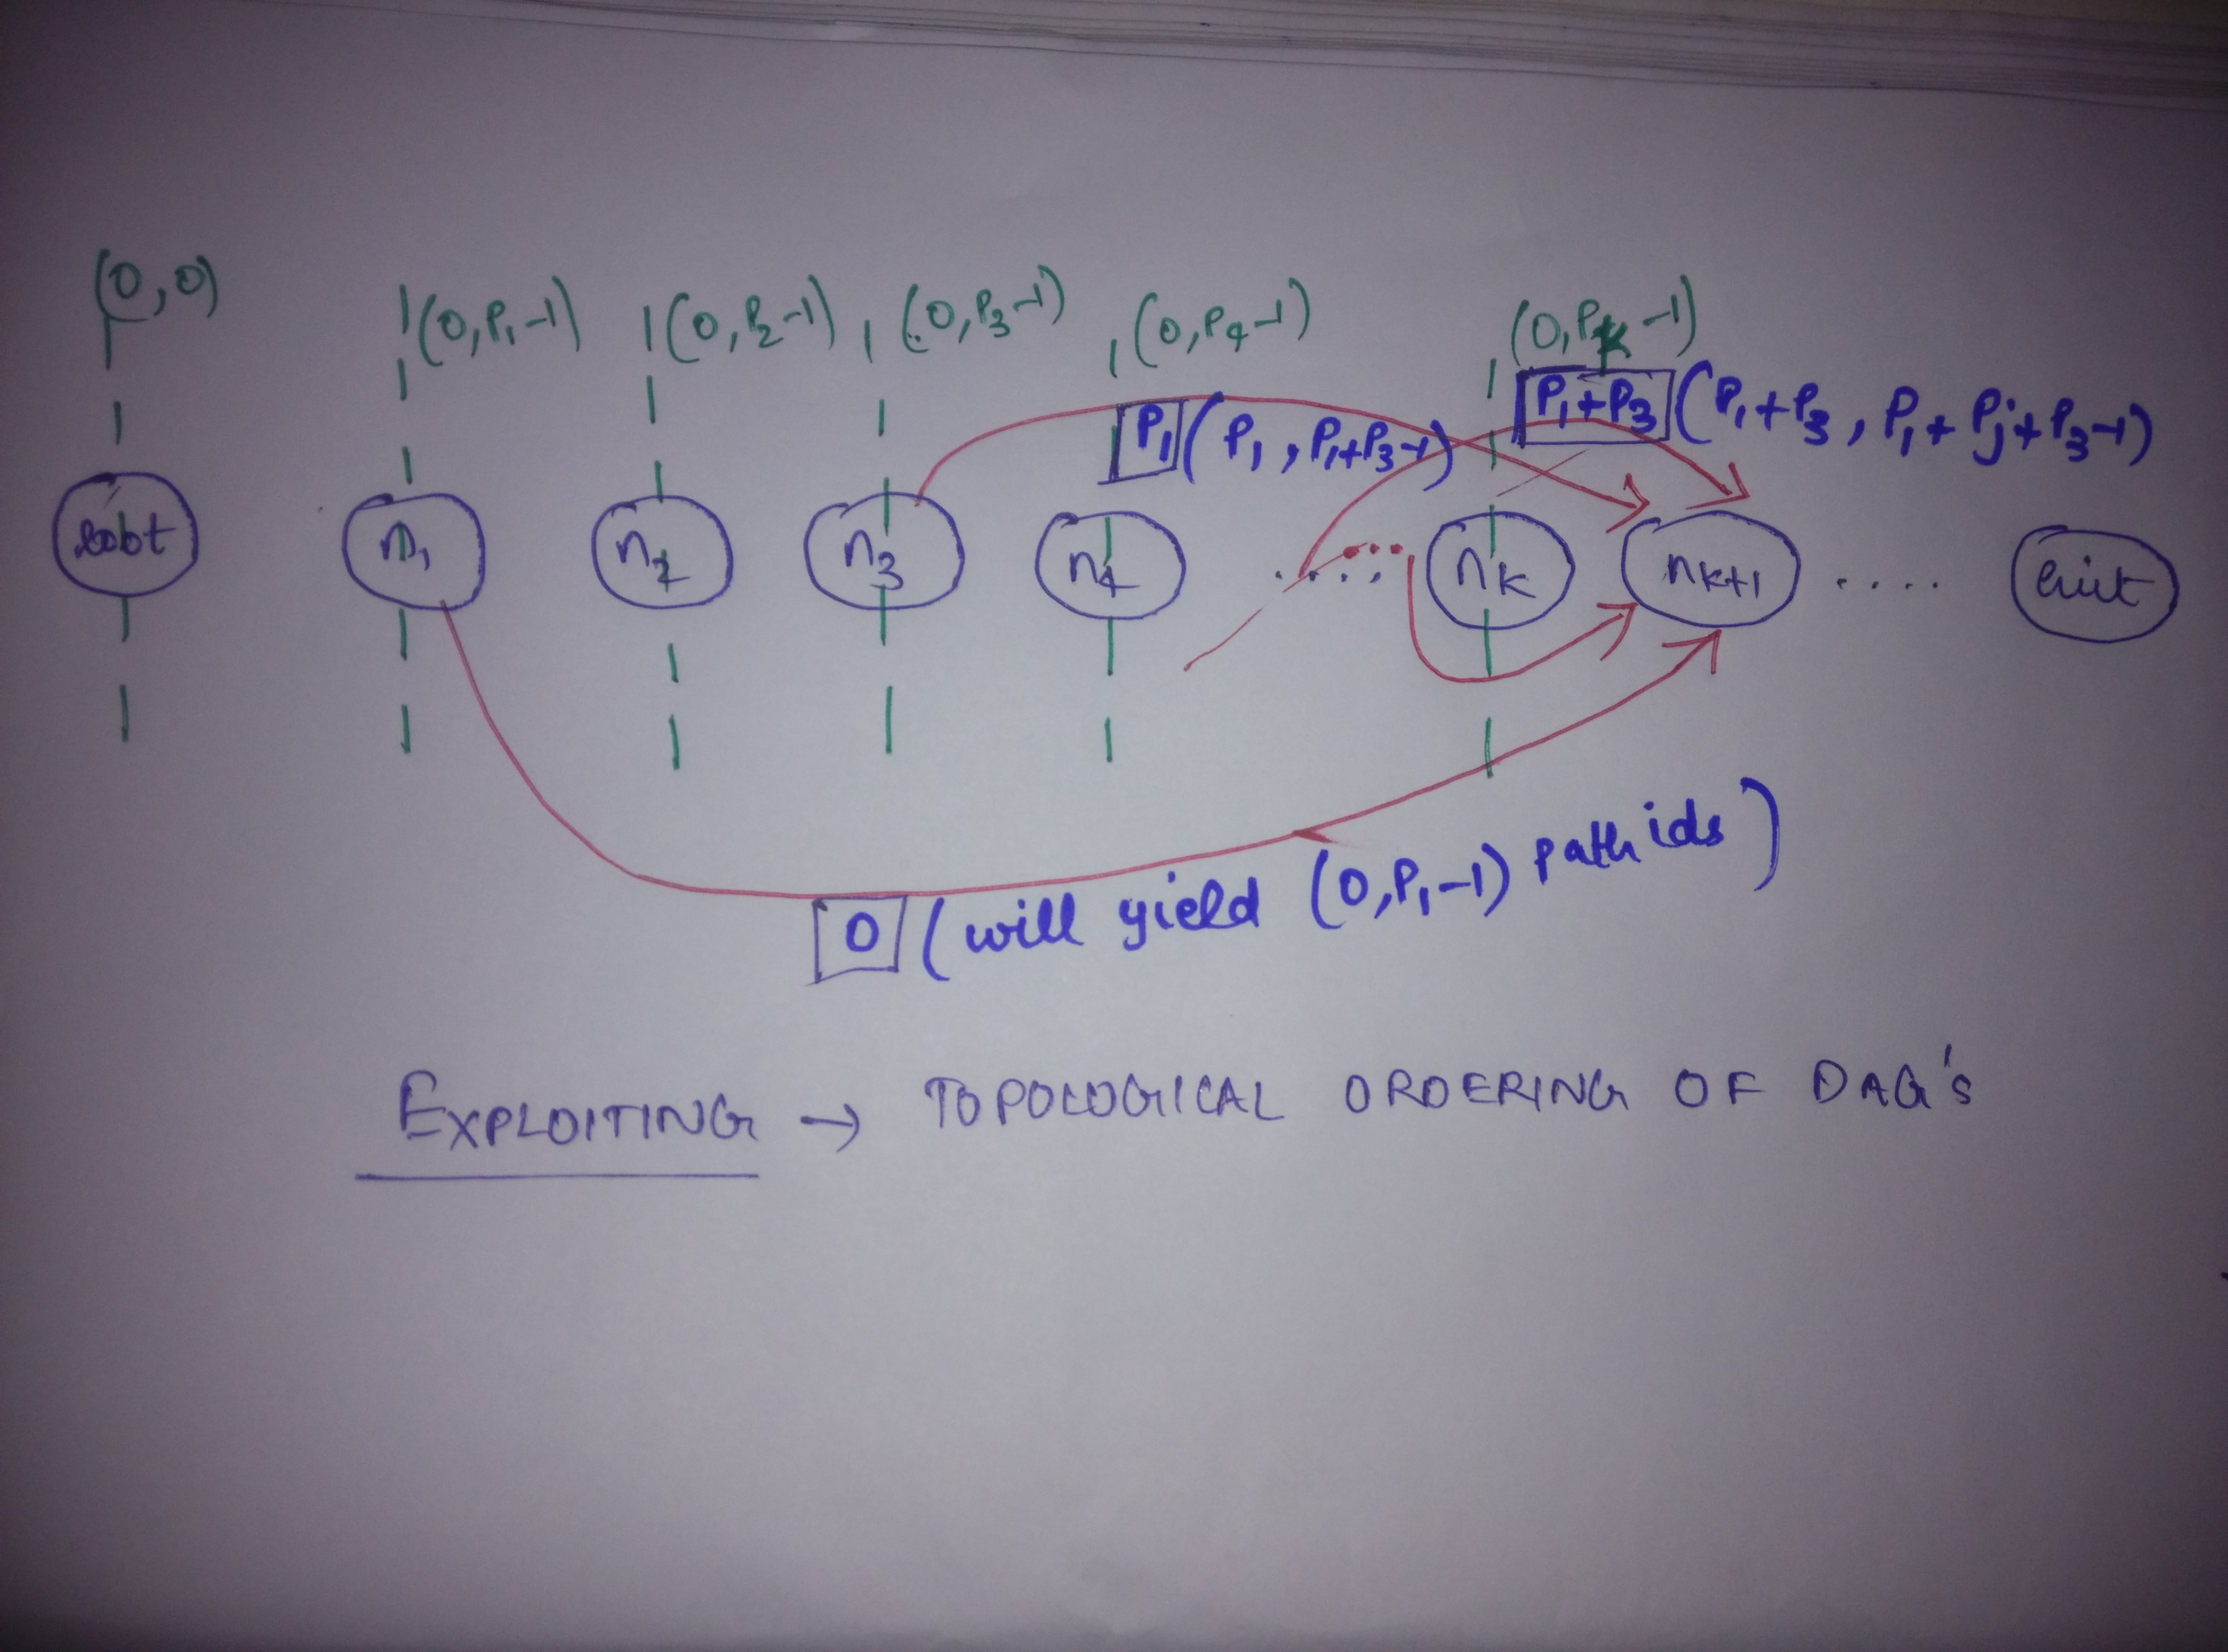
\includegraphics[scale=0.09]{3.jpg}
\end{center}
Then chose, the PM cabin's as shown above. This way just by adding one more commando, on $p_2$ facing towards ${Square}_1$, we can exhaust our required full square! \\*
Thus, proved by induction. \\*
Note, this has to be an optimal solution as we are ensuring that every box is guarded by just one commando (this is because of the combine step which does not disturb any guarded box and the base case for which the claim holds). 
\end{document}
